% chapters/chapter2/2_4_lqr_design.tex
% !TeX root=../../main.tex

\section{طراحی کنترل‌کننده تنظیم‌گر خطی درجه دوم (\lr{LQR})}

به منظور پایدارسازی سیستم حول نقطه تعادل و ایجاد یک معیار ارزیابی (\lr{Benchmark}) برای مقایسه با کنترل‌کننده‌های پیشرفته‌تر، در گام نخست یک کنترل‌کننده فیدبک حالت بهینه از نوع تنظیم‌گر خطی درجه دوم (\lr{LQR}) طراحی می‌شود. همان‌گونه که در تحلیل ژاکوبین به اثبات رسید، تغییر طول کابل در تقریب خطی فاقد اثرگذاری دینامیکی است. بر این اساس، در این فاز طول کابل ثابت فرض شده ($l = l_0 = 0.5\mathrm{\ m}$) و مکانیزم وینچ غیرفعال در نظر گرفته می‌شود ($\dot{l} = 0 , \ddot{l} = 0$). در نتیجه، تنها عملگر فعال سیستم، نیروی محرک ارابه ($F$) است و ماتریس توزیع ورودی ($B_{\mathrm{LQR}}$) به ستون اول ماتریس $B$ تقلیل می‌یابد:
\begin{equation}
    \renewcommand{\arraystretch}{1.8}
    B_{\mathrm{LQR}} = \begin{bmatrix} 0 \\ \frac{1}{M} \\ 0 \\ -\frac{1}{M l_0} \end{bmatrix}
\end{equation}

تئوری کنترل \lr{LQR} بر پایه حداقل‌سازی یک تابع هزینه بی‌نهایت-افق (\lr{Infinite-Horizon Cost Function}) به فرم درجه دوم بنا شده است. این تابع هزینه، تعادلی بهینه میان خطای حالت (انحراف از نقطه تعادل) و تلاش کنترلی (انرژی مصرفی عملگرها) ایجاد می‌کند:
\begin{equation}
    J = \int_{0}^{\infty} \left( x^T Q x + u^T R u \right) dt
\end{equation}
که در آن، $x$ بردار حالت سیستم، $u$ سیگنال کنترلی (نیروی $F$)، $Q \ge 0$ ماتریس نیمه‌معین مثبت وزن حالات و $R > 0$ پارامتر معین مثبت وزن ورودی است. با توجه به مقادیر پارامترهای فیزیکی سیستم ($M=1\mathrm{\ kg}$، $m=0.2\mathrm{\ kg}$، $g=9.81\mathrm{\ m/s^2}$ و ضرایب اصطکاک مفصلی)، ماتریس‌های وزن بر اساس اهمیت متغیرهای کنترلی به صورت زیر تنظیم می‌شوند:
\begin{align}
    Q & = \mathrm{diag}([1000, 10, 500, 10]) \\
    R & = 1
\end{align}

درایه $Q_{11} = 1000$ نشان‌دهنده جریمه سنگین بر خطای موقعیت کالسکه ($x$) است تا سیستم با سرعت بالایی به نقطه هدف همگرا شود. همچنین، درایه $Q_{33} = 500$ به منظور اعمال قید نرم بر زاویه آونگ ($\theta$) و سرکوب نوسانات انتخاب شده است. وزن‌های متناظر با سرعت‌ها ($Q_{22}, Q_{44}$) در مقادیر پایین‌تری تنظیم شده‌اند تا از رفتار نوسانی شدید جلوگیری شود. انتخاب $R=1$ نیز اجازه می‌دهد تا کنترل‌کننده از ظرفیت عملگر نیرو به نحو مطلوب بهره‌برداری کند.

قانون کنترل بهینه به فرم فیدبک حالت $u = -Kx$ تعریف می‌شود. ماتریس بهره فیدبک ($K$) از طریق حل معادله جبری ریکاتی (\lr{Algebraic Riccati Equation}) محاسبه می‌گردد:
\begin{equation}
    A^T P + P A - P B_{\mathrm{LQR}} R^{-1} B_{\mathrm{LQR}}^T P + Q = 0
\end{equation}
\begin{equation}
    K = R^{-1} B_{\mathrm{LQR}}^T P
\end{equation}

با حل این معادله برای پارامترهای سیستم مورد مطالعه، ماتریس بهره بهینه $K$ به صورت زیر استخراج می‌شود:
\begin{equation}
    K = \begin{bmatrix} 31.6228 & 14.0488 & -17.7264 & 0.3611 \end{bmatrix}
\end{equation}

سیگنال کنترلی نهایی تولید شده توسط این استراتژی برابر با $F = -Kx$ است. شماتیک معماری حلقه بسته این کنترل‌کننده در شکل \ref{fig:lqr_block} نشان داده شده است. این ساختار مدار-بسته، مبنای ارزیابی عملکرد سیستم در مواجهه با شرایط اولیه و خطاهای موقعیت مختلف در فصل شبیه‌سازی خواهد بود.

\begin{figure}[htbp]
    \centering
    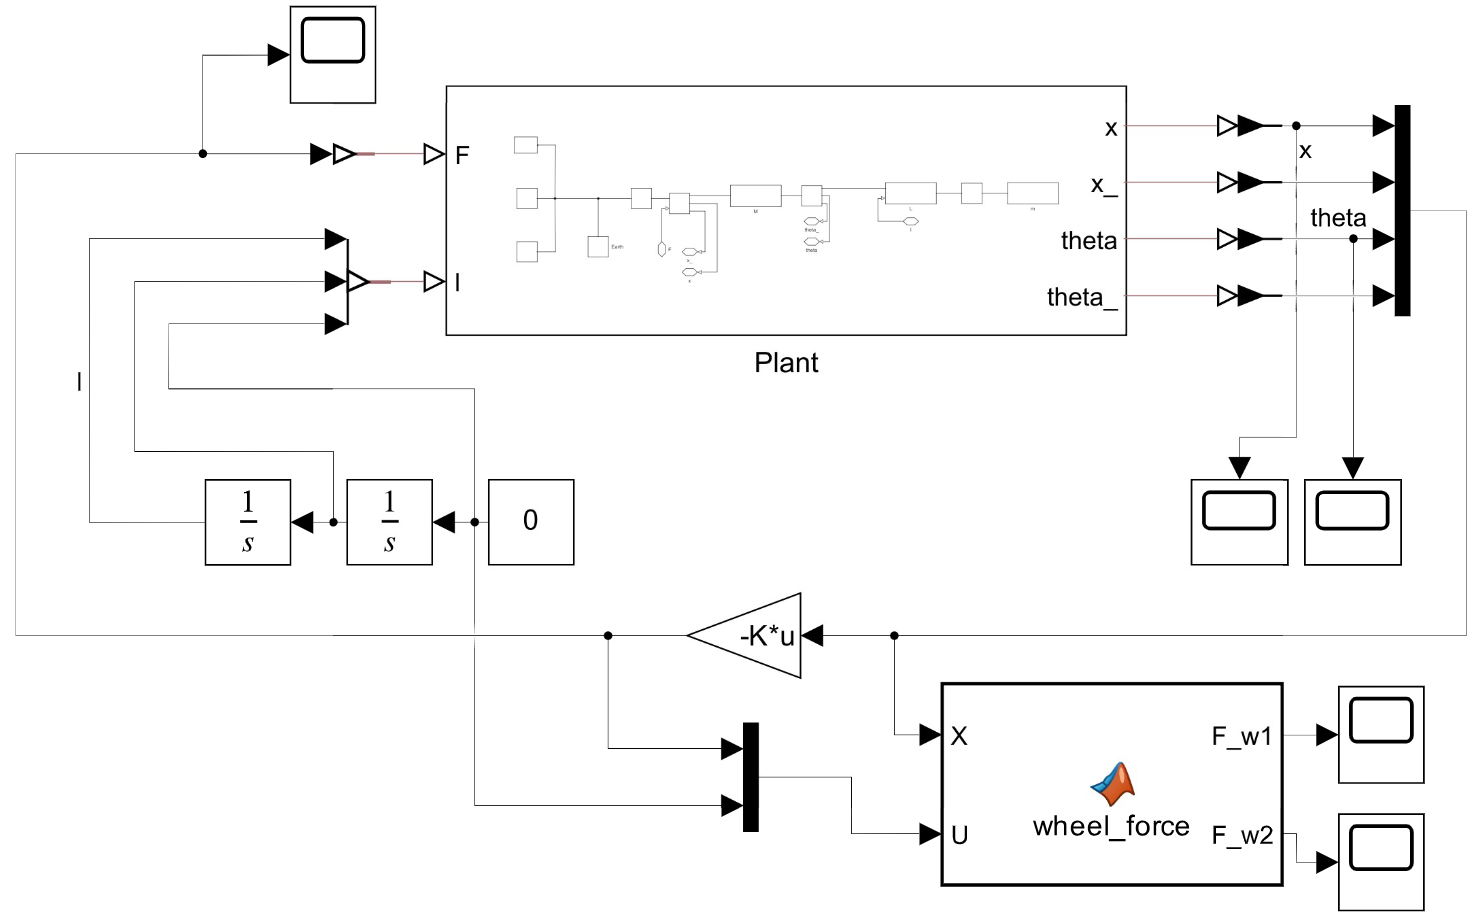
\includegraphics[width=0.8\textwidth]{images/1_LQR_Step/LQR_block_diagram.png}
    \caption{معماری حلقه بسته کنترل‌کننده خطی \lr{LQR} با فرض طول کابل ثابت.}
    \label{fig:lqr_block}
\end{figure}